%%******************************************************************************
%%
%% introduction.tex
%%
%%******************************************************************************
%%
%% Title......: Introduction
%%
%% Author.....: GSCAR-DFKI
%%
%% Started....: Nov 2013
%%
%% Emails.....: alcantara@poli.ufrj.br elael@poli.ufrj renan028@gmail.com
%%
%% Address....: Universidade Federal do Rio de Janeiro
%%              Caixa Postal 68.504, CEP: 21.945-970
%%              Rio de Janeiro, RJ - Brasil.
%%
%%******************************************************************************


%%******************************************************************************
%% SECTION - Eletronica
%%******************************************************************************

\section{Proposta 3 – PC embarcado e PC na base}

\subsection{Arquitetura da Eletrônica Proposta 3}
A terceira solução consiste em realizar tanto um processamento na eletrônica
embarcada, quanto na base. Poderá ser utilizado tanto uma eletrônica importada
com Pelican Case quanto uma solução semelhante a 2, com PC104, e um laptop a
base. Observar a figura~\ref{prop3}.

\begin{figure}[H]
    \centering
    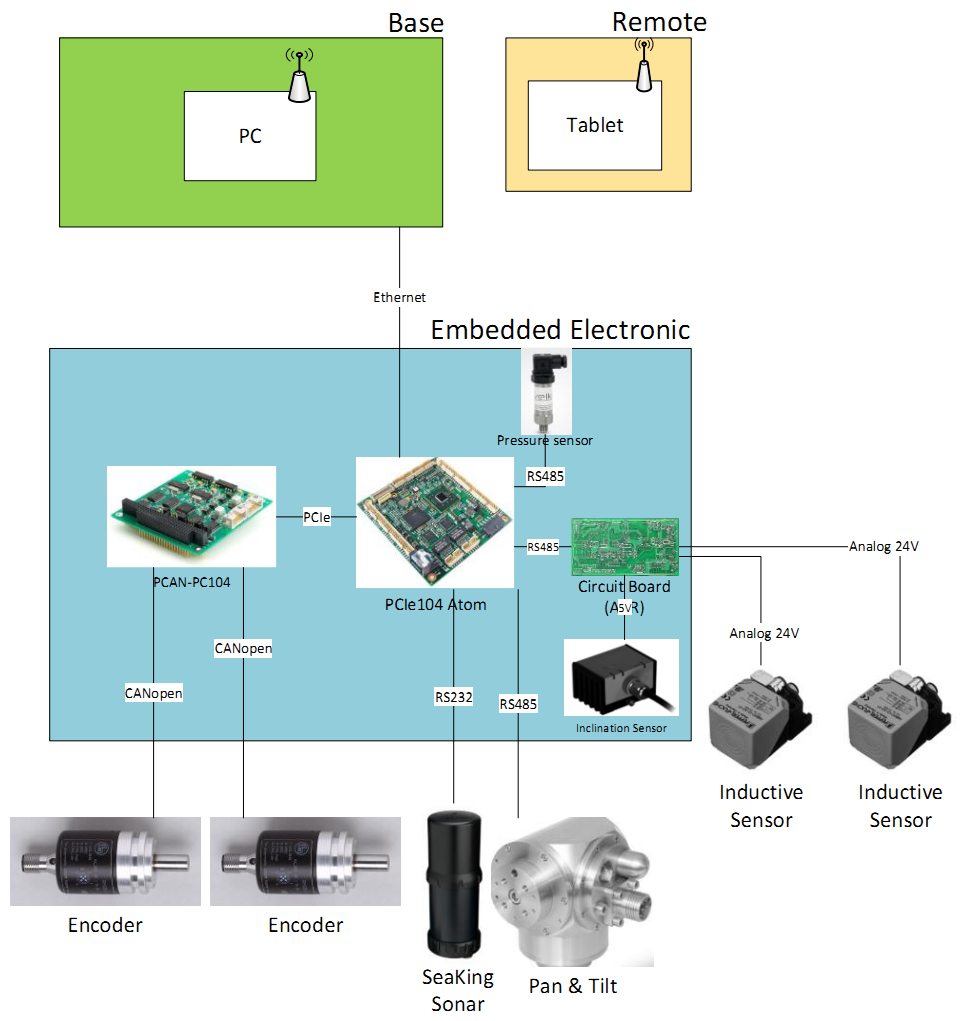
\includegraphics[width=0.5\columnwidth]{figs/eletronica/5.png}
    \caption{Diagrama de Comunicações - Proposta 3}
    \label{prop3}
\end{figure} 

\subsection{Arquitetura de Software Proposta 3}
Esta proposta é um meio termo entre a proposta com todo o processamento em terra
(proposta 1) e a proposta anterior, na qual todo o processamento de dados se dá
na eletrônica embarcada, figura \ref{fig:FL:3}. Os componentes de software são
basicamente os mesmos, excetuando-se a ordem em que o processamento e a comunicação ocorrem.


\afterpage{
\begin{landscape}
\begin{figure}
\centering
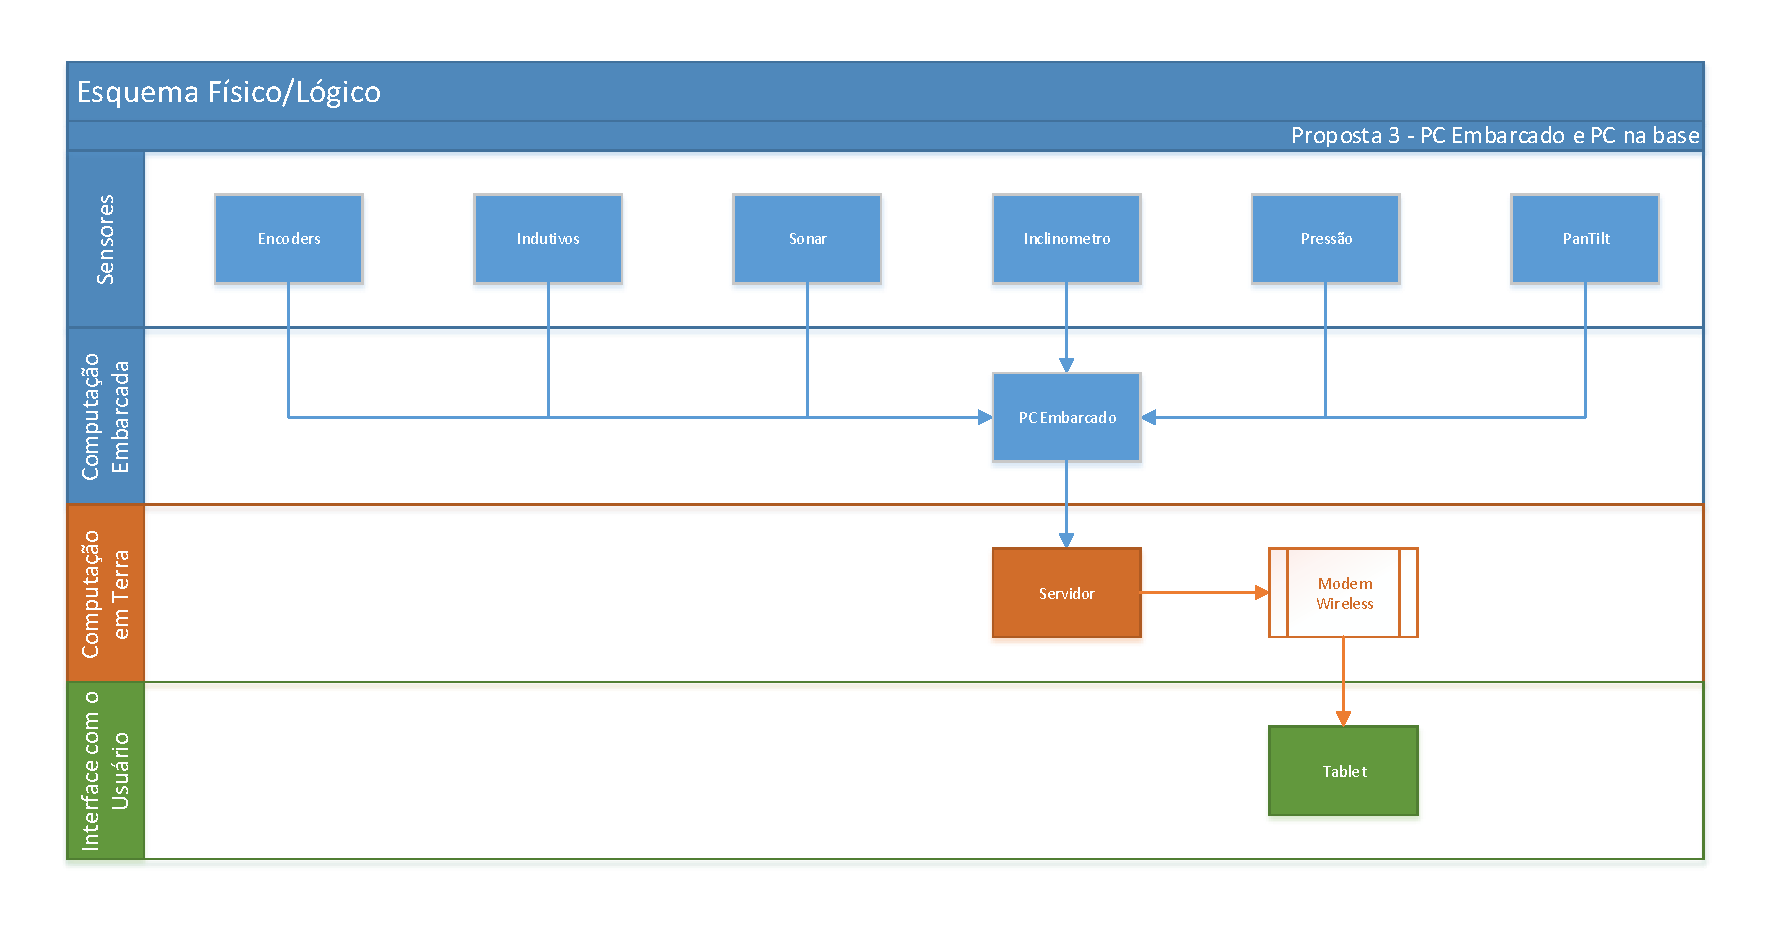
\includegraphics[width=1\linewidth,keepaspectratio]{figs/software/LogicoFisico/EsqLogicoFisico3n.pdf}
\caption{Relação entre os componentes físicos e as divisões lógicas da
proposta 3.}
\label{fig:FL:3}
\end{figure}
\end{landscape}
}


\begin{figure}[H]
\centering
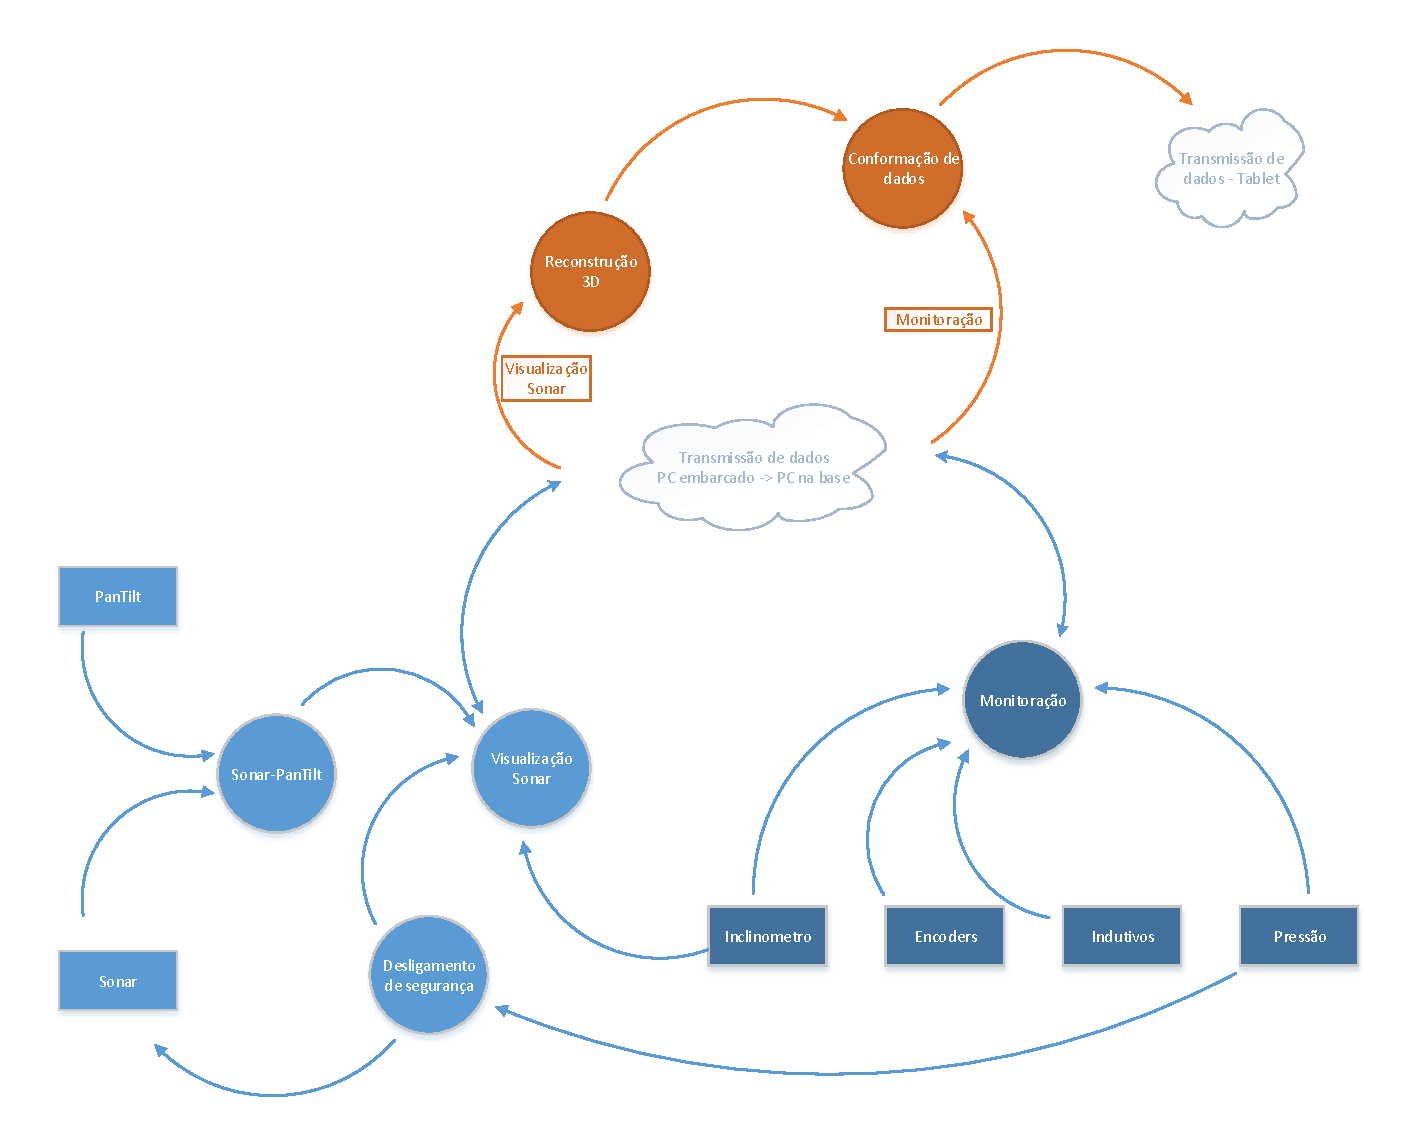
\includegraphics[width=\textwidth,height=\textheight,keepaspectratio]{figs/software/EstrutSoft/prop1_soft_3.pdf}
\caption{Interconexões entre os componentes de software da proposta 3.}
\label{fig:ES:3}
\end{figure}

Os dados dos sensores das operações de inserção e remoção de Stoplogs (encoders,
inclinômetro, sensores indutivos e sensor de pressão), assim como os dados
brutos provenientes do sonar e do módulo PanTilt serão conformados e fundidos em
um computador embarcado e enviados via ethernet para um computador em
superfície, componentes azuis da figura \ref{fig:ES:3}. O componente de
segurança do sonar também estará presente.



Já na superfície os dados do componente Sonar-PanTilt serão processados pelo
módulo de reconstrução 3D que irá gerar a imagem, analogamente as outras
propostas, componentes laranjas da figura \ref{fig:ES:3}.
Por fim os componentes de Monitoração e Visualiza\-ção enviarão os dados
processados para o tablet.

A maior vantagem dessa arquitetura, na ótica de software, é a facilidade de
manutenção, uma vez que para a realização de qualquer alteração do software do
sistema não é necessário a abertura da envólucro do sistema embarcado. Já a sua
desvantagem seria a maior quantidade de trabalho para a programação de dois
sistemas.